% Auto generated LaTeX figure include file.
% Copy selected blocks into your Overleaf report.

\begin{figure}[H]
    \centering
    
\includegraphics[width=0.92\textwidth]{figures/Fig01_Current_Time.png}
    \caption{Fig01 Current Time.}
    \label{fig:fig01:current:time}
\end{figure}

\begin{figure}[H]
    \centering
    
\includegraphics[width=0.92\textwidth]{figures/Fig02_CoilForce_Time.png}
    \caption{Fig02 CoilForce Time.}
    \label{fig:fig02:coilforce:time}
\end{figure}

\begin{figure}[H]
    \centering
    
\includegraphics[width=0.92\textwidth]{figures/Fig03_Weight_Time.png}
    \caption{Fig03 Weight Time.}
    \label{fig:fig03:weight:time}
\end{figure}

\begin{figure}[H]
    \centering
    
\includegraphics[width=0.92\textwidth]{figures/Fig04_NetForce_Time.png}
    \caption{Fig04 NetForce Time.}
    \label{fig:fig04:netforce:time}
\end{figure}

\begin{figure}[H]
    \centering
    
\includegraphics[width=0.92\textwidth]{figures/Fig05_Displacement_Time.png}
    \caption{Fig05 Displacement Time.}
    \label{fig:fig05:displacement:time}
\end{figure}

\begin{figure}[H]
    \centering
    
\includegraphics[width=0.92\textwidth]{figures/Fig06_SynchronizedSignals_Time.png}
    \caption{Fig06 SynchronizedSignals Time.}
    \label{fig:fig06:synchronizedsignals:time}
\end{figure}

\begin{figure}[H]
    \centering
    
\includegraphics[width=0.92\textwidth]{figures/Fig07_TriggerZoom_0_30ms.png}
    \caption{Fig07 TriggerZoom 0 30ms.}
    \label{fig:fig07:triggerzoom:0:30ms}
\end{figure}

\begin{figure}[H]
    \centering
    
\includegraphics[width=0.92\textwidth]{figures/Fig08_Force_Current.png}
    \caption{Fig08 Force Current.}
    \label{fig:fig08:force:current}
\end{figure}

\begin{figure}[H]
    \centering
    
\includegraphics[width=0.92\textwidth]{figures/Fig09_Displacement_Current.png}
    \caption{Fig09 Displacement Current.}
    \label{fig:fig09:displacement:current}
\end{figure}

\begin{figure}[H]
    \centering
    
\includegraphics[width=0.92\textwidth]{figures/Fig10_Force_Displacement.png}
    \caption{Fig10 Force Displacement.}
    \label{fig:fig10:force:displacement}
\end{figure}

\begin{figure}[H]
    \centering
    
\includegraphics[width=0.92\textwidth]{figures/Fig11_LSTM_Displacement_Prediction.png}
    \caption{Fig11 LSTM Displacement Prediction.}
    \label{fig:fig11:lstm:displacement:prediction}
\end{figure}

\begin{figure}[H]
    \centering
    
\includegraphics[width=0.92\textwidth]{figures/Fig12_LSTM_Force_Prediction.png}
    \caption{Fig12 LSTM Force Prediction.}
    \label{fig:fig12:lstm:force:prediction}
\end{figure}

\begin{figure}[H]
    \centering
    
\includegraphics[width=0.92\textwidth]{figures/Fig13_LSTM_Prediction_Errors.png}
    \caption{Fig13 LSTM Prediction Errors.}
    \label{fig:fig13:lstm:prediction:errors}
\end{figure}

\begin{figure}[H]
    \centering
    
\includegraphics[width=0.92\textwidth]{figures/Fig14_LSTM_TriggerZoom.png}
    \caption{Fig14 LSTM TriggerZoom.}
    \label{fig:fig14:lstm:triggerzoom}
\end{figure}

\begin{figure}[H]
    \centering
    
\includegraphics[width=0.92\textwidth]{figures/Fig15_Report_Data_Summary.png}
    \caption{Fig15 Report Data Summary.}
    \label{fig:fig15:report:data:summary}
\end{figure}

\begin{figure}[H]
    \centering
    
\includegraphics[width=0.92\textwidth]{figures/Fig16_LSTM_Normalized_Sequences.png}
    \caption{Fig16 LSTM Normalized Sequences.}
    \label{fig:fig16:lstm:normalized:sequences}
\end{figure}

\begin{figure}[H]
    \centering
    
\includegraphics[width=0.92\textwidth]{figures/Fig17_LSTM_Model_Workflow.png}
    \caption{Fig17 LSTM Model Workflow.}
    \label{fig:fig17:lstm:model:workflow}
\end{figure}

\begin{figure}[H]
    \centering
    
\includegraphics[width=0.92\textwidth]{figures/Fig20_LSTM_Training_RMSE_History.png}
    \caption{Fig20 LSTM Training RMSE History.}
    \label{fig:fig20:lstm:training:rmse:history}
\end{figure}

\begin{figure}[H]
    \centering
    
\includegraphics[width=0.92\textwidth]{figures/Fig21_LSTM_Training_Loss_History.png}
    \caption{Fig21 LSTM Training Loss History.}
    \label{fig:fig21:lstm:training:loss:history}
\end{figure}

\begin{figure}[H]
    \centering
    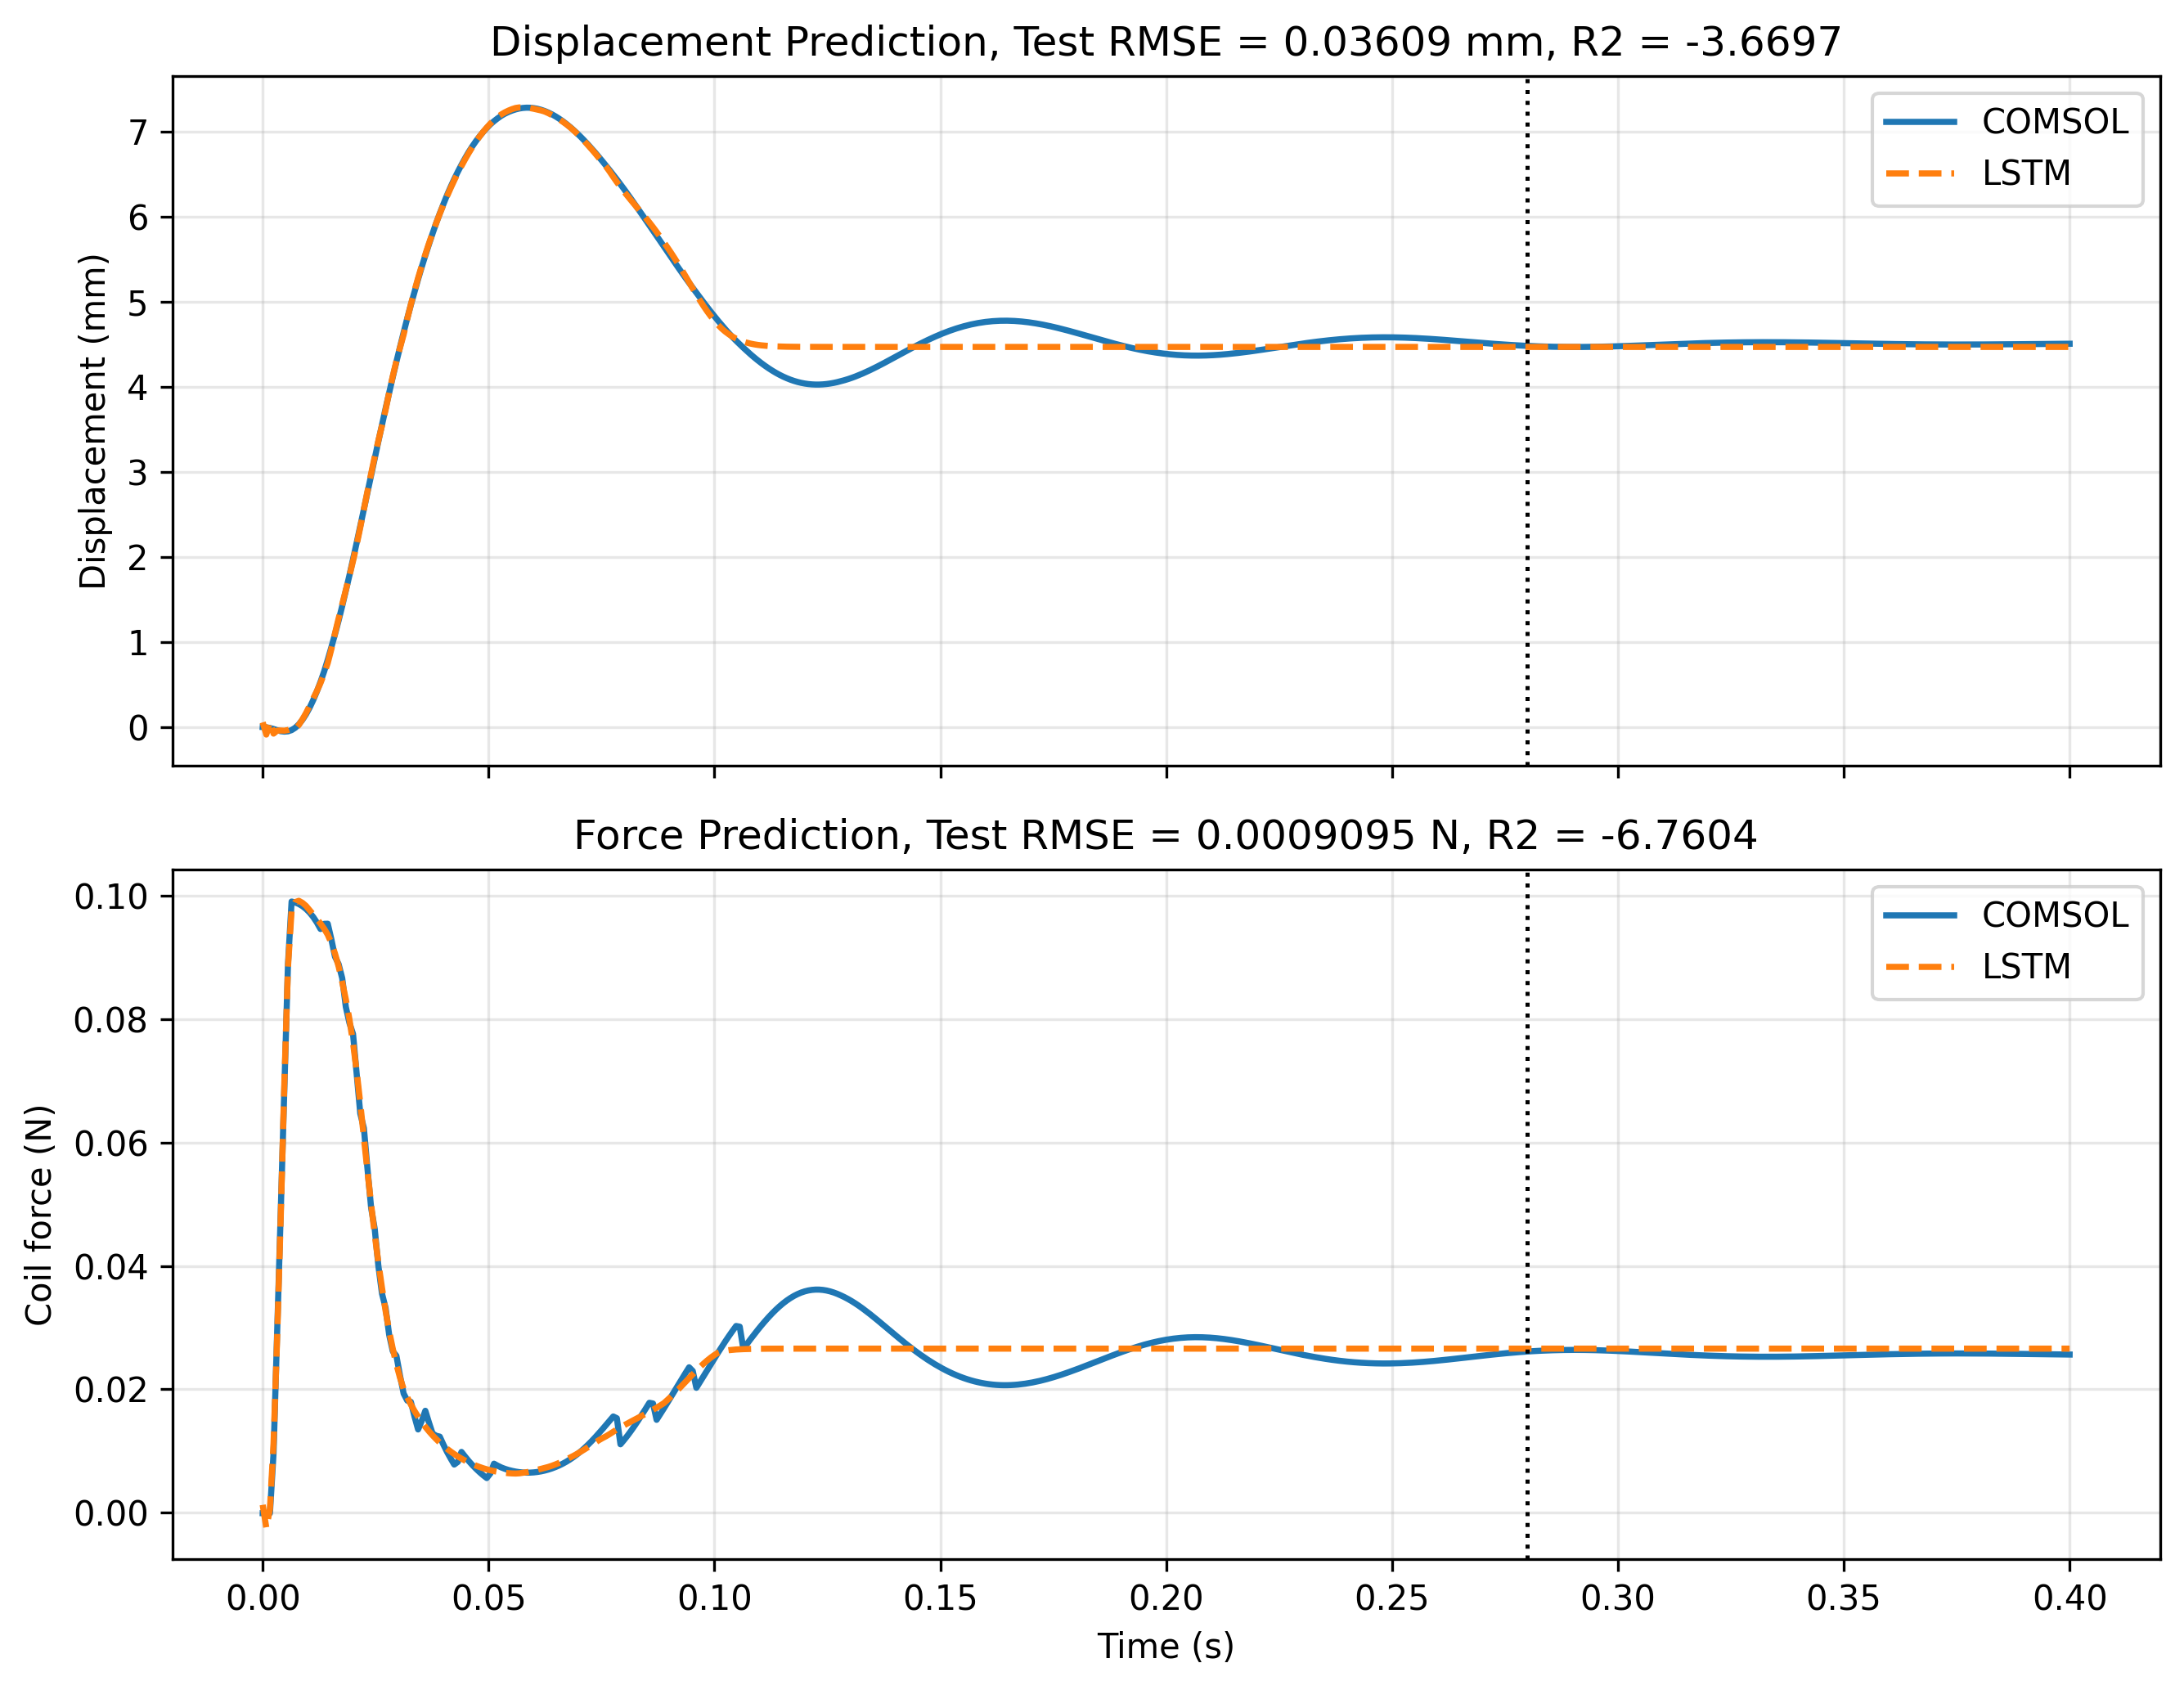
\includegraphics[width=0.92\textwidth]{figures/Fig22_LSTM_Accuracy_Time_Response.png}
    \caption{Fig22 LSTM Accuracy Time Response.}
    \label{fig:fig22:lstm:accuracy:time:response}
\end{figure}

\begin{figure}[H]
    \centering
    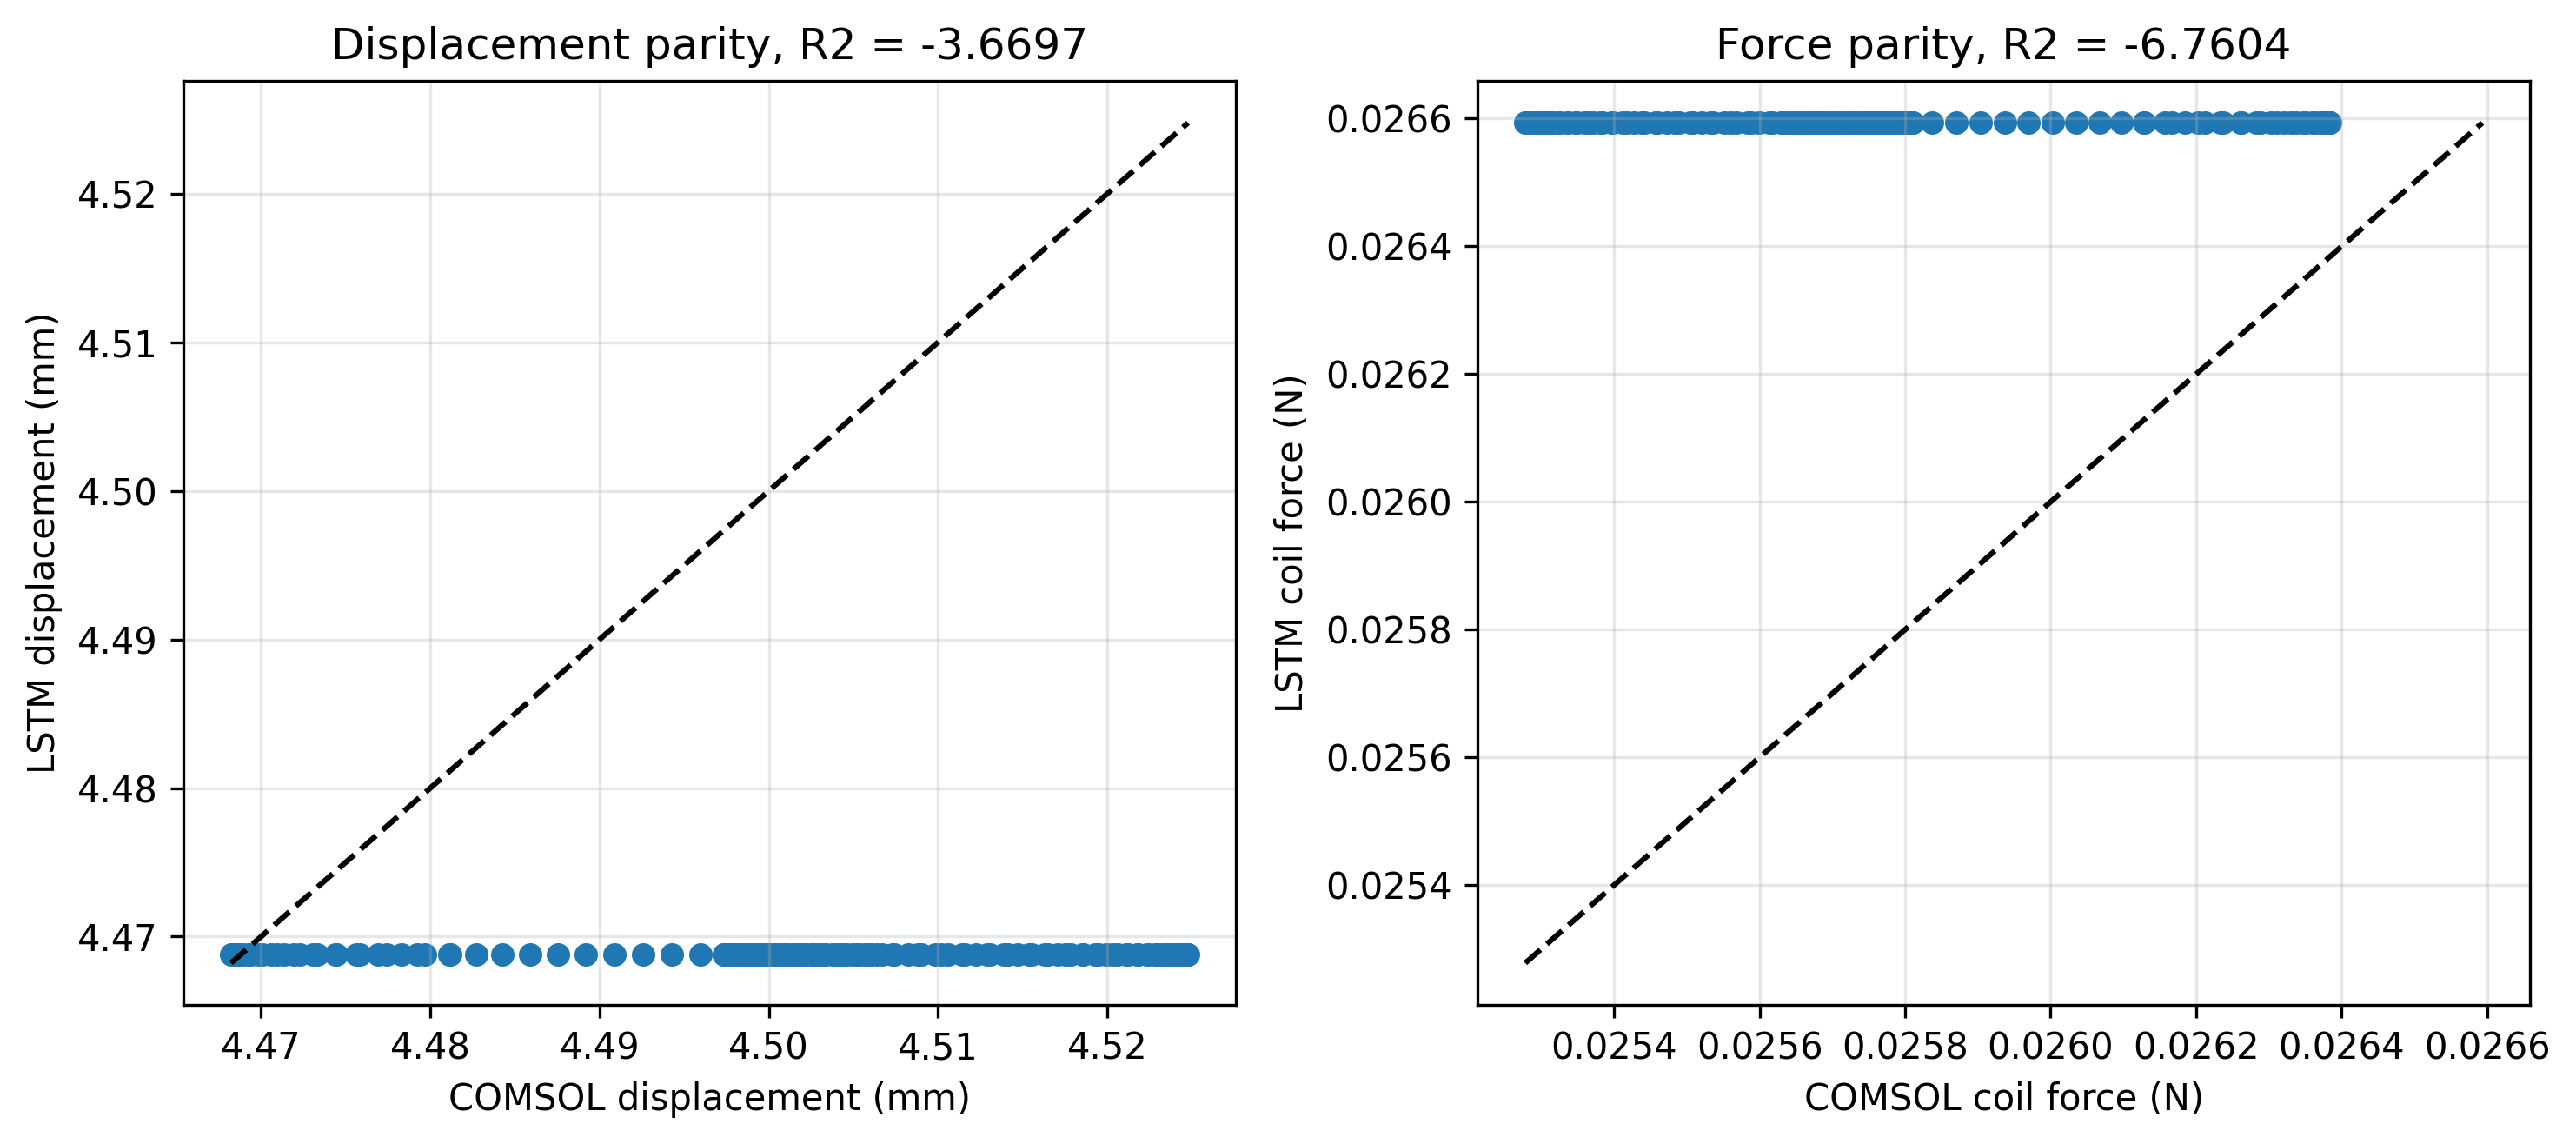
\includegraphics[width=0.92\textwidth]{figures/Fig23_LSTM_Accuracy_Parity_Plots.png}
    \caption{Fig23 LSTM Accuracy Parity Plots.}
    \label{fig:fig23:lstm:accuracy:parity:plots}
\end{figure}

\begin{figure}[H]
    \centering
    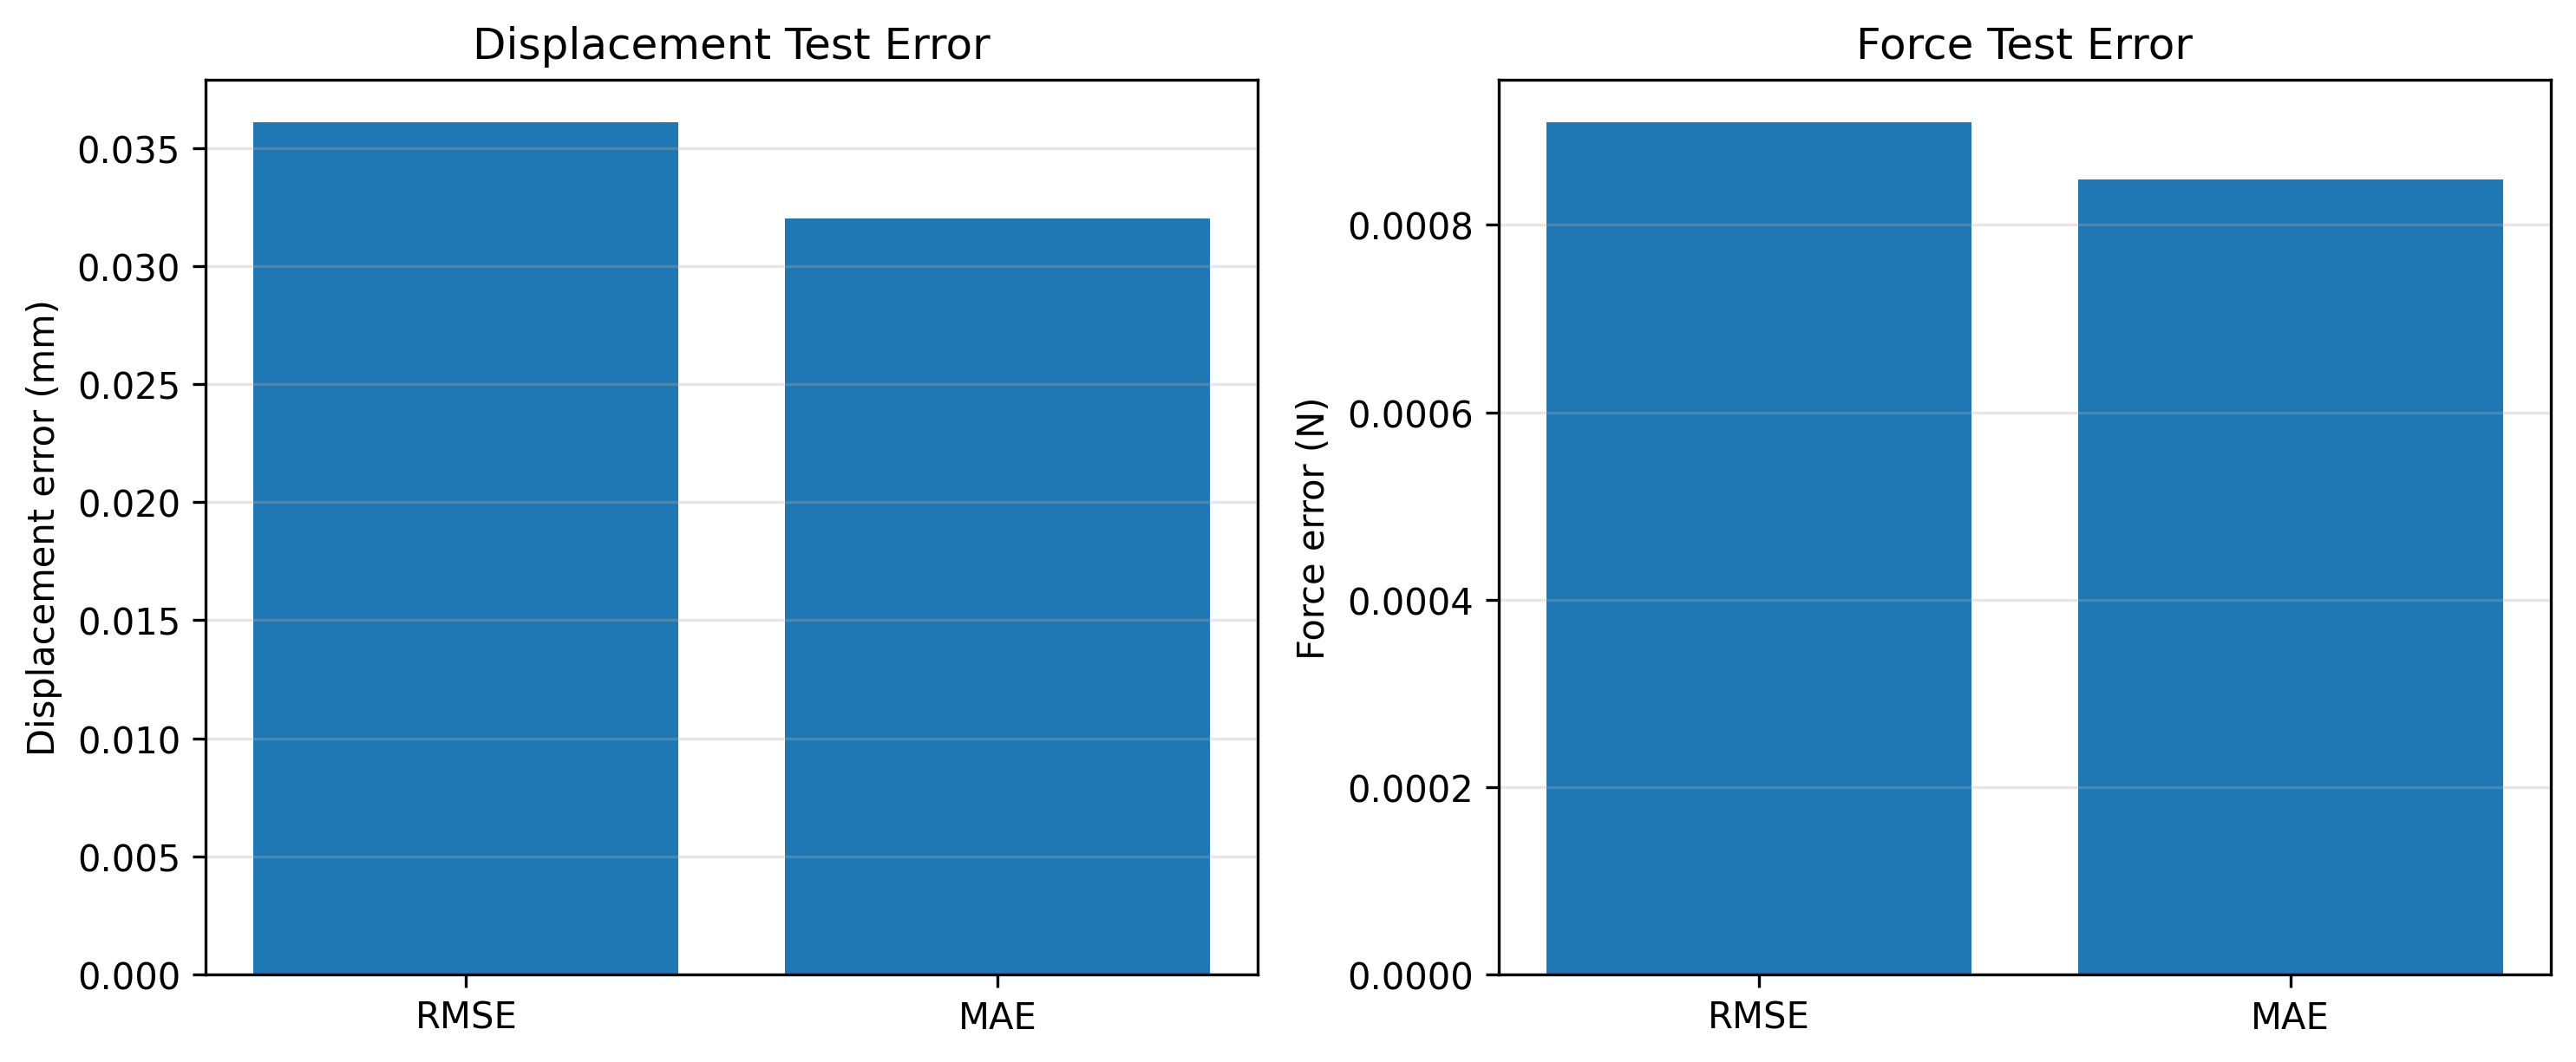
\includegraphics[width=0.92\textwidth]{figures/Fig24_LSTM_Test_Accuracy_Metrics.png}
    \caption{Fig24 LSTM Test Accuracy Metrics.}
    \label{fig:fig24:lstm:test:accuracy:metrics}
\end{figure}

